%%%%%%%%%%%%%%%%%%%%%%%%%%%%%%%%%%%%%%%%%%%%%%%%%%%%%%%%%%%%%%%%%
%%% %
%%% % weiiszablon.tex
%%% % The Faculty of Electrical and Computer Engineering
%%% % Rzeszow University Of Technology diploma thesis Template
%%% % Szablon pracy dyplomowej Wydziału Elektrotechniki 
%%% % i Informatyki PRz
%%% % June, 2015
%%%%%%%%%%%%%%%%%%%%%%%%%%%%%%%%%%%%%%%%%%%%%%%%%%%%%%%%%%%%%%%%%

\documentclass[12pt,twoside]{article}

\usepackage{weiiszablon}
\usepackage{tikz}
\usetikzlibrary{shapes.geometric}
\usetikzlibrary{shapes.misc}
\usetikzlibrary{shapes.symbols}
\usepackage{array}
\usepackage{tabularx}
\usepackage{booktabs}
\usepackage{multirow}

\author{Jakub Maternia}

% np. EF-123456, EN-654321, ...
\studentID{179956}

\title{Dla punktów płaszczyzny, o współrzędnych x i y zapisanych w tablicach, znaleźć ich najbliższych sąsiadów.}


%%% promotor
\supervisor{(dr inż. prof. PRz ) Mariusz Borkowski}
%% przykład: dr hab. inż. Józef Nowak, prof. PRz








% strona tytułowa
\begin{document}
\maketitle

\clearpage

\tableofcontents

\clearpage

\section{Treść zadania}

9. Dla punktów płaszczyzny, których współrzędne x i y są przechowywane w dwóch tablicach o długości n utwórz tablicę, która pod i-tym indeksem będzie przechowywać indeks najbliższego sąsiada i-tego punktu.
\\ Przykład:
\begin{lstlisting}[caption=Przykład,label={Przyklad}]
wejscie: 0, 1, -2, -1, 10 
		 	   0, 2, -3, -10, 9
wyjscie: 1, 0, 0, 2, 1
  \end{lstlisting}


\section{Podejście brute force}
\subsection{Analiza problemu i potencjalne rozwiązanie}
Problem polega na obliczeniu odległości pomiędzy punktami oraz porównania jej z każdą inną wartością w poszukiwaniu najmniejszej dla danego punktu.
Rozwiązanie polega na "wzięciu" jednego punktu oraz policzeniu jego odległości do każdego innego punku oraz znalezieniu najmniejszej i zapisaniu indeksu.
Ta metoda rozwiąże ten problem niezależnie od sytuacji, sprawdzi wszystkie możliwe przypadki.
W sytuacji kiedy wybrane zostaną dwa takie same punkty, program powinien wybrać inny od tego który został "wyciągnięty", stąd sprawdzanie czy indeksy są różne pomiędzy dwoma punktami.
Zainicjowana tablica index i wypełniona wartościami -1, aby mieć pewność, że indeksy zapisują się odpowiednio zostanie wypełniona wartościami zmiennej in, w której będzie zapisywany indeks punktu o najmniejszej odległości.
Na końcu zostanie zwrócona tablica i wypisana na ekran.\\
Danymi wejściowymi będą dwie tablice tabx i taby oraz długość tych tablic zapisana w zmiennej n, a danymi wyjściowymi będzie tablica index.
\clearpage
\subsection{Schemat blokowy}
        \begin{center}
            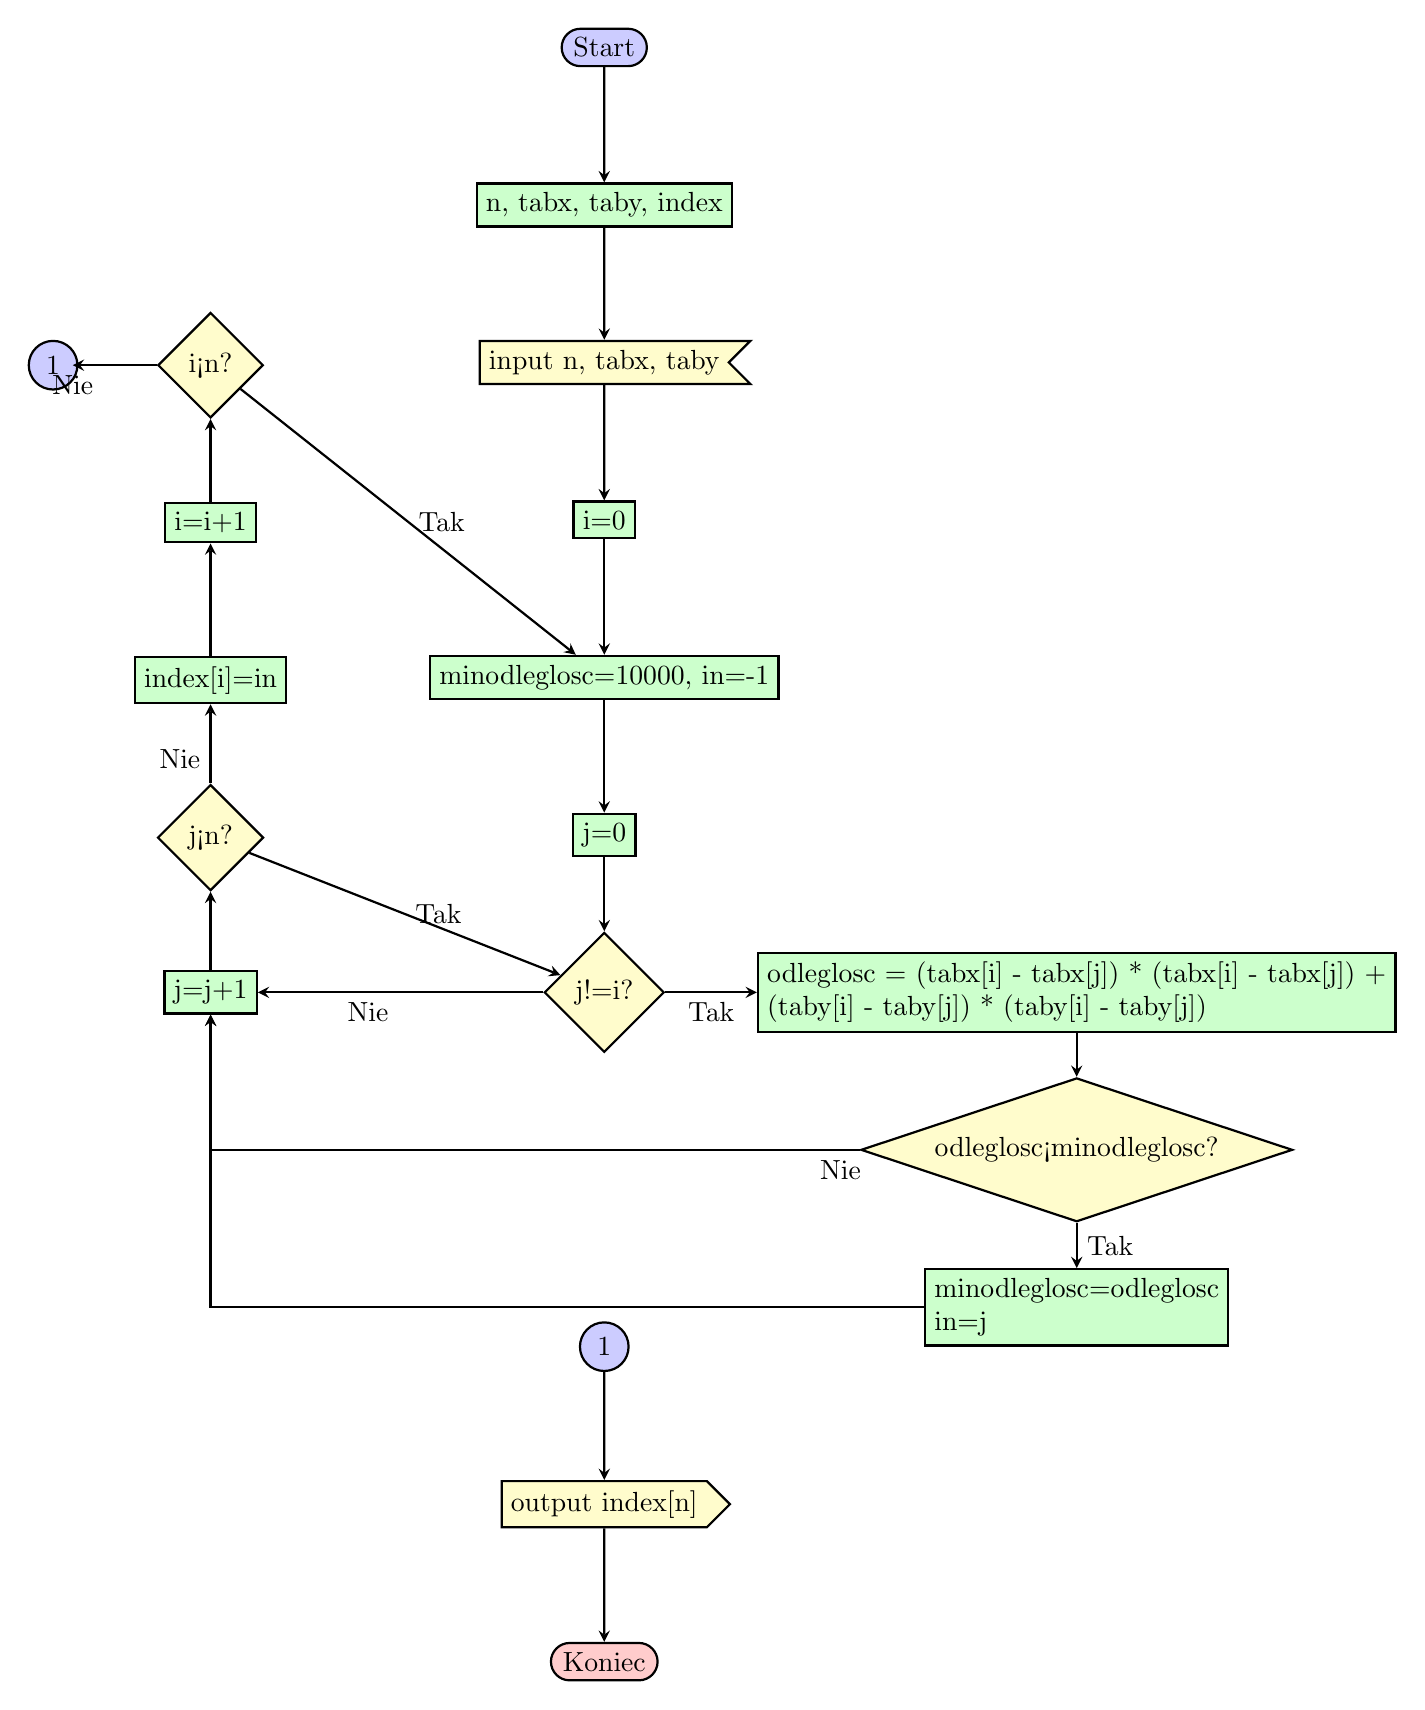
\begin{tikzpicture}[node distance=2cm, thick, >=stealth]  % Definiowanie obrazka tworzonego dzięki środowisku Tikz
                % Punkty decyzyjne
                \node (start) [rounded rectangle, draw, fill=blue!20] {Start};
                \node (process) [rectangle, draw, below of=start, fill=green!20] {n, tabx, taby, index};
                \node (process1) [signal, signal from=east, signal to=nowhere, draw, below of=process, fill=yellow!20] {input n, tabx, taby};
                \node (process2) [rectangle, draw, fill=green!20, below of=process1] {i=0};
                \node (process3) [rectangle, draw, fill=green!20, below of=process2] {minodleglosc=10000, in=-1};
                \node (process4) [rectangle, draw, fill=green!20, below of=process3] {j=0};
                \node (process5) [diamond, draw, fill=yellow!20, below of=process4] {j!=i?};
                \node (process6) [rectangle, draw, fill=green!20, left of=process5, xshift=-3cm] {j=j+1};
                \node (process7) [rectangle, draw, fill=green!20, right of=process5, align=left, xshift = 4cm] {odleglosc = (tabx[i] - tabx[j]) * (tabx[i] - tabx[j]) + \\(taby[i] - taby[j]) * (taby[i] - taby[j])};
                \node (process8) [diamond, draw, fill=yellow!20, below of=process7, aspect=3] {odleglosc<minodleglosc?};
                \node (process9) [diamond, draw, fill=yellow!20, above of=process6, yshift=-1] {j<n?};
                \node (process10) [rectangle, draw, fill=green!20, below of=process8, align=left] {minodleglosc=odleglosc\\in=j};
                \node (process11) [rectangle, draw, fill=green!20, above of=process9] {index[i]=in};
                \node (process12) [rectangle, draw, fill=green!20, above of=process11] {i=i+1};
                \node (process13) [diamond, draw, fill=yellow!20, above of=process12] {i<n?};
                \node (process14) [circle, draw, fill=blue!20, left of=process13] {1};
                \node (process15) [circle, draw, fill=blue!20, below of=process5, yshift=-2.5cm] {1};
                \node (process16) [signal, signal from=nowhere, signal to=east, draw, below of=process15, fill=yellow!20] {output index[n]};
                \node (end) [rounded rectangle, draw, below of=process16,, fill=red!20] {Koniec};
                
                % Strzałki
                \draw[->] (start) -- (process);
                \draw[->] (process) -- (process1);
                \draw[->] (process1) -- (process2);
                \draw[->] (process2) -- (process3);
                \draw[->] (process3) -- (process4);
                \draw[->] (process4) -- (process5);
                \draw[->] (process5) -- node[right, anchor=north] {Tak} (process7);
                \draw[->] (process5) -- ++(-3,0) node[left, anchor=north] {Nie} |- (process6);
                \draw[->] (process6) -- (process9);
                \draw[->] (process7) -- (process8);
                \draw[->] (process8) -- node[right] {Tak} (process10);
                \draw[->] (process8) -- ++(-3,0) node[left, anchor=north] {Nie} -| (process6);
                \draw[->] (process10) -| (process6);

                \draw[->] (process9) -- node[right] {Tak} (process5);
                \draw[->] (process9) -- ++(0,1) node[left] {Nie} -| (process11);
                \draw[->] (process11) -- (process12);
                \draw[->] (process12) -- (process13);
                \draw[->] (process13) -- node[right] {Tak} (process3);
                \draw[->] (process13) -- ++(-1.75,0) node[left, anchor=north] {Nie} (process14);

                \draw[->] (process15) -- (process16);
                \draw[->] (process16) -- (end);
                %\draw[->] (process1) -- node[right] {Tak} (end);
                %\draw[->] (process1) -- ++(-3,0) node[left] {Nie} |- (process);
            \end{tikzpicture}
        \end{center}
\clearpage

\subsection{Pseudokod}
\begin{lstlisting}[language=C++,caption=Pseudokod BruteForce,label={pseudokodbrute}]
input: n, tabx, taby
output: index
index := -1
dla i od 0 do n-1 wykonaj
    minodleglosc := 10000
    in := -1
dla j od 0 do n-1 wykonaj
    jesli i != j wtedy
        odleglosc := (tabx[i] - tabx[j]) * (tabx[i] - tabx[j]) + (taby[i] - taby[j]) * (taby[i] - taby[j])
        jesli odleglosc < minodleglosc wtedy
            minodleglosc:= odleglosc
            in := j
        koniec jesli
    koniec jesli
koniec dla
index[i] := in
koniec dla
zwroc index
\end{lstlisting}


\subsection{Przykładowe rozwiązanie}
\begin{table}[ht]
    \centering
    \begin{tabularx}{\textwidth}{|c|c|c|c|c|c|c|X|}
        \hline
        \textbf{i} & \textbf{j} & \textbf{punkt[i]} & \textbf{punkt[j]} & \textbf{odleglosc} & \textbf{minodleglosc} & \textbf{in} & \textbf{index} \\
        \hline
        0 & 1 & 0,0 & 1,2 & 2,23 & 2,23 & 1 & 1, -1, -1, -1 \\
        \hline
        0 & 2 & 0,0 & -2,-3 & 3,61 & 2,23 & 1 & 1, -1, -1, -1 \\
        \hline
        0 & 3 & 0,0 & -1,-10 & 10,04 & 2,23 & 1 & 1, -1, -1, -1 \\
        \hline
        1 & 0 & 1,2  & 0,0 & 2,23 & 2,23 & 0 & 1, 0, -1, -1 \\
        \hline
        1 & 2 & 1,2  & -2,-3 & 5,83 & 2,23 & 0 & 1, 0, -1, -1 \\
        \hline
        1 & 3 & 1,2  & -1,-10 & 12,16 & 2,23 & 0 & 1, 0, -1, -1 \\
        \hline
        2 & 0 & -2,-3  & 0,0 & 3,06 & 3,06 & 0 & 1, 0, 0, -1 \\
		\hline
        2 & 1 & -2,-3  & 1,2 & 5,83 & 3,06 & 0 & 1, 0, 0, -1 \\
		\hline
        2 & 3 & -2,-3  & -1,-10 & 7,07 & 3,06 & 0 & 1, 0, 0, -1 \\
		\hline
        3 & 0 & -1,-10  & 0,0 & 10,04 & 10,04 & 0 & 1, 0, 0, 0 \\
        \hline
        3 & 1 & -1,-10  & 1,2 & 12,16 & 10,04 & 0 & 1, 0, 0, 0 \\
		\hline
        3 & 2 & -1,-10  & -2,-3 & 7,07 & 7,07 & 2 & 1, 0, 0, 2\\
		\hline
    \end{tabularx}
    \caption{Przykładowe rozwiązanie BruteForce.}
    \label{tab:bruteforceprzyklad}
\end{table}

\subsection{Złożoność obliczeniowa}
Złożoność obliczeniowa tego algorytmu wynosi \(O(n^2)\), wynika to z faktu sprawdzania każdego punktu (oprócz tego samego). 
Program wykonuje porównanie i-tego elementu z j-tym elementem, gdzie jest ich n-1.
Dokonujemy więc \(n\cdot(n-1)\) porównań co ostatecznie daje nam złożonośc na poziomie: \(n^2-n-1\).\\
Zatem złożoność czasowa algorytmu jest skategoryzowana jako \(O(n^2)\).



\section{Druga metoda z wykorzystaniem metody dziel i zwyciężaj}
\subsection{Metoda działania}
Jeśli chcemy przyspieszyć działanie programu należy zająć się ilością dokonywanych operacji obliczania odległości. 
Dzieląc wejście do sytuacji kiedy mamy 2 lub 3 punkty możemy ograniczyć liczbę liczenia odległości i niskim kosztem stwierdzić indeks którego punktu jest najbliżej. 
Jednak zanim to będzie możliwe trzeba ułożyć dane w taki sposób żeby choć w małej części punkty leżały blisko siebie np. sortując po wartości współrzędnej x.
Tym sposobem otrzymamy punkty, których indeksy najbliższych sąsiadów są obok siebie.
Jeśli to nie nastąpi, podczas procesu scalania należy sprawdzić pas graniczny wokół granicy podziału o długości \(2\cdot{d}\).
Wtedy porównamy graniczne punkty z obu stron granicy podziału tak aby upewnić się czy przypadkiem po drugiej stronie granicy nie leży punkt, który jest bliższy niż ten, który wcześniej został oznaczony jako najbliższy wewnątrz podzielonego zbioru.
Dzięki właściwościom geometrii ograniczamy liczbę porównań do maksymalnie 7 punktów dla każdego punktu w pasie granicznym.
Wynika to z faktu, że punkty w pasie są rozłożone w taki sposób, że mogą zajmować maksymalnie 7 sąsiednich komórek w siatce kwadratów o długości d/2.
Żeby otrzymać wynik wystarczy będzie scalić spowrotem podzbiory oraz ustawić tablicę przechowującą odpowiedzi w odpowiedni sposób - tak aby wartości odzwierciedlały te, które zostały podane wcześniej.
\clearpage
\subsection{Schemat blokowy}

\begin{figure}[h!]
    \centering
    \hspace{-17cm}
    \makebox[0pt][l]{\includegraphics[scale = 0.55]{schematmet2w1.png}}
\end{figure}
\clearpage
\begin{figure}[h!]
    \centering
    \hspace{-19cm}
    \makebox[0pt][l]{\includegraphics[scale = 0.5]{schematmet2w2.png}}
    \caption{\label{fig:schematmet2}Schemat blokowy dla drugiej metody rozwiązania problemu.}
\end{figure}
\clearpage
\subsection{Pseudokod}
\begin{lstlisting}[language=C++,caption=Pseudokod Dziel i zwyciężaj,label={pseudokoddivide}]
    input: punkty, n
    output: index
    jesli n <= 1 wtedy
        zwroc []
    koniec jesli
    
    posortuj punkty wedlug wspolrzednej x
    wykonaj podzial(punkty, 0, n-1, index)
    zwroc index
    
    funkcja podzial(punkty, lewa, prawa, index)
        jesli prawa - lewa + 1 <= 3 wtedy
            zwroc bruteForce(punkty, lewa, prawa, index)
        koniec jesli
        
        mid := (lewa + prawa) / 2
        granica_lewa := podzial(punkty, lewa, mid, index)
        granica_prawa := podzial(punkty, mid+1, prawa, index)
        d := min(granica_lewa, granica_prawa)
        
        scal(punkty, lewa, mid, prawa, d, index)
        zwroc d
    koniec funkcji
    
    funkcja scal(punkty, lewa, mid, prawa, d, index)
        granica := []
        dla i od lewa do prawa wykonaj
            jesli abs(punkty[i].x - punkty[mid].x) < d wtedy
                dodaj punkty[i] do granica
            koniec jesli
        koniec dla
        
        posortuj granica wedlug wspolrzednej y
        dla i od 0 do rozmiar(granica) - 1 wykonaj
            dla j od i+1 do min(i+8, rozmiar(granica)) wykonaj
                jesli granica[j].y - granica[i].y >= d wtedy
                    przerwij
                koniec jesli
                
                odleglosc := sqrt((granica[i].x - granica[j].x)^2 + (granica[i].y - granica[j].y)^2)
                jesli odleglosc < d wtedy
                    zaktualizuj index dla granica[i] oraz granica[j]
                    d := odleglosc
                koniec jesli
            koniec dla
        koniec dla
    koniec funkcji
    
    funkcja bruteForce(punkty, lewa, prawa, index)
        dla i od lewa do prawa wykonaj
            minodleglosc := nieskonczonosc
            dla j od lewa do prawa wykonaj
                jesli i != j wtedy
                    odleglosc := sqrt((punkty[i].x - punkty[j].x)^2 + (punkty[i].y - punkty[j].y)^2)
                    jesli odleglosc < minodleglosc wtedy
                        minodleglosc := odleglosc
                        index[i] := j
                    koniec jesli
                koniec jesli
            koniec dla
        koniec dla
        zwroc minodleglosc
    koniec funkcji

    \end{lstlisting}

\clearpage
\subsection{Przykładowe rozwiązanie}
Przejdźmy przez kroki rozwiązania tego problemu na przykładzie, używając takich danych: \\
tabx = {1, 3, 5, 2} i taby = {2, 4, 1, 2}.\\
\textbf{Krok 1:} Przygotowanie tablicy index = {-1, -1, -1, -1}\\
\textbf{Krok 2:} Przeniesienie danych do tablicy punkty i posortowanie rosnąco względem współrzędnej x.\\
punkty = [(1, 2), (2, 2), (3, 4), (5, 1)]\\
\textbf{Krok 3:} Rekurencyjne dzielenie tablicy punkty na mniejsze podzbiory. Lewa część: (1,2), (2,2). Prawa część: (3,4), (5,1).\\
\textbf{Krok 4:} Obliczenie odległości w lewej części metodą Bruteforce (nie dzielimy na mniejsze podzbiory ponieważ liczba punktów jest mniejsza niż 3).\\
\textbf{Krok 5:} Zapisanie odpowiedzi do tablicy indeks: indeks[0] = 1, indeks[1] = 0.\\
\textbf{Krok 6:} Analogicznie dla prawej części: indeks[2] = 3, indeks[3] = 2.\\
\textbf{Krok 7:} Scalanie, sprawdzenie czy w pasie granicznym wokół granicy podziału znajdują się punkty, które mogą mieć mniejszą odległość.\\
\(2\cdot{d}\) = 2 (minimalna odległość pomiędzy punktami w obu częściach pomnożona x2). \\
\textbf{Krok 8:} Sprawdzenie odległości pomiędzy punktami, które znajdują się od siebie w takiej o
Odległość pomiędzy punktami (2,2) i (3,4) wynosi 2,24. Jest większa niż \(2\cdot(d)\) więc wynik się nie zmienia.\\
\textbf{Krok 9:} Wypisanie tablicy indeks = [1, 0, 3, 2].


\subsection{Złożoność obliczeniowa}
Ponieważ w tym algorytmie obliczamy odległość metodą Brute-Force tylko dla dwóch lub trzech punktów, złożoność obliczeniowa tego procesu w najgorszym przypadku to \(O(n)\), ponieważ jeden punkt jest najbliższym sąsiadem drugiego i odwrotnie. \\
Sortowanie względem współrzędnej x jest dokonywane poprzez funkcję sort z biblioteki algorithm, którego złożoność obliczeniowa to \(O(n\cdot(log(n))\)). Podobnie dla scalania, którego złożoność to również \(O(n\cdot(log(n))\)). \\
Zatem złożoność całego algorytmu to również \(O(n\cdot(log(n))\)).


\section{Implementacja obu algorytmów}
\subsection{Testy wydajności}
\begin{table}[h!]
    \centering
    \begin{tabular}{|c|c|c|c|c|c|}
    \hline
    $n$ & 1000 & 5000 & 10000 & 15000 & 20000 \\ \hline
    Brute & 0.004492s & 0.175671s & 0.59253s7 & 1.15787s & 2.11035s \\ \hline
    Divide & 0s & 0.004499s & 0.010095s & 0.011432s & 0.001563s \\ \hline
    \end{tabular}
    \caption{Porównanie czasów dla algorytmów Brute Force i Divide dla różnych wartości $n$.}
    \label{tab:porownanie}
\end{table}

\begin{figure}[h!]
    \centering
    \includegraphics[width=1\linewidth]{zlozonosc.png}
    \caption{\label{fig:zlozonosc}Wykres złożoności czasowej, porównujący dwie metody.}
\end{figure}

Algorytm wykorzystujący metodę dziel i zwyciężaj wykazał się niesamowitą wydajnością, nawet dla dużych rozmiarów danych, dokładnie tak jak w założeniu.



\clearpage
\subsection{Kody programów}
\subsubsection{BruteForce}
\begin{lstlisting}[language=C++,caption=Kod BruteForce,label={bruteforcekod}]
    #include <iostream>
    #include <cmath>
    #include <ctime>
    #include <chrono>
    #include <fstream>
    #include <cassert>
    
    using namespace std;
    
    int* szukanie(int n, int* tabx, int* taby){
        int *index = new int[n];    // Deklaracja tablicy index
        double odleglosc=0;
        
        for (int i =0; i<n;i++){   // Uzupelnienie tablicy index wartosciami -1 aby miec pewnosc ze nie beda mialy wplyw na wynik
            index[i]=-1;
        }	
        for (int i = 0; i<n;i++){   // Obliczanie i zapisywanie indeksow najblizszych sasiadow
            double minodleglosc=numeric_limits<double>::infinity();
            int in=-1;
            for (int j = 0; j<n; j++){
                if (j!=i){
                odleglosc = (tabx[i] - tabx[j]) * (tabx[i] - tabx[j]) + (taby[i] - taby[j]) * (taby[i] - taby[j]);
                if (odleglosc < minodleglosc) {
                    minodleglosc = odleglosc;
                    in = j;				
                    }
                }
            }
            index[i]=in;		
        }
        
        return index;
    }
    
    void testy() {   // Funkcja przeprowadzajaca testy przy uzyciu assert
        // Test 1: Prosty przypadek
        int tabx1[] = {0, 1, 2};
        int taby1[] = {0, 0, 0};
        int n1 = 3;
        int* wynik1 = szukanie(n1, tabx1, taby1);
        assert(wynik1[0] == 1);
        assert(wynik1[1] == 0 || wynik1[1] == 2);
        assert(wynik1[2] == 1);
        delete[] wynik1;
    
        // Test 2: Punkty w pionie
        int tabx2[] = {0, 0, 0};
        int taby2[] = {0, 1, 2};
        int n2 = 3;
        int* wynik2 = szukanie(n2, tabx2, taby2);
        assert(wynik2[0] == 1);
        assert(wynik2[1] == 0 || wynik2[1] == 2);
        assert(wynik2[2] == 1);
        delete[] wynik2;
    
        // Test 3: Jeden punkt
        int tabx3[] = {5};
        int taby3[] = {5};
        int n3 = 1;
        int* wynik3 = szukanie(n3, tabx3, taby3);
        assert(wynik3[0] == -1);
        delete[] wynik3;
        
        cout <<endl <<  "Test OK";
    }
    
    
    int main(){
        
        ifstream file("danebrute.txt");   // Obsluga otwierania pliku
        if (!file.is_open()) {
            cout << "Nie udalo sie otworzyc pliku" << endl;
            return 1;
        }
        
        int n;
        file >> n;  // Pobieranie liczby punktow z pliku
        //cout << "Wpisz ilosc punktow: " << endl;
        //cin >> n;
        
        if (n <= 0) {
            cout << "Liczba punktow musi byc dodatnia!" << endl;
            return 1;
        }
        
        int *tabx = new int[n];   // Deklaracja tablic
        int *taby = new int[n];
        int *index;    // Deklaracja wskaznika do tablicy index, ktora jest stworzona w funkcji
        
        srand(time(NULL));
        
        for(int i = 0; i<n; i++){   // Uzupelnienie tablic
            //tabx[i] = rand() % 10;
            //taby[i] = rand() % 10;
            file >> tabx[i];
        }
        for(int i = 0; i<n; i++){
            file >> taby[i];
        }
        
        for(int i = 0;i<n;i++){   // Wypisanie tablic na ekran
            cout << tabx[i] << " ";
        }
        
        cout << endl;
        
        for(int i = 0;i<n;i++){
            cout << taby[i] << " ";
        }
        
        cout << endl;
        file.close();  // Zamkniecie pliku -> dane zostaly przepisane do tablic
        std::chrono::high_resolution_clock::time_point t1 = std::chrono::high_resolution_clock::now();
        index = szukanie(n,tabx, taby);	// Przypisanie wskaznika do tablicy "zwrotnej" z funkcji szukanie
        std::chrono::high_resolution_clock::time_point t2 = std::chrono::high_resolution_clock::now();
        
        std::chrono::duration<double> time_span = std::chrono::duration_cast<std::chrono::duration<double>>(t2 - t1);
        
        for (int i=0; i<n;i++){  // Wypisanie wyniku na ekran
            cout << index[i] << " ";
        }
        
        testy();  // Wywolanie funkcji w ktorej wykonywane sa testy
        
        cout << endl << "czas: " << time_span.count() << endl;  // Wypisanie pomiaru czasu
        
        delete[] tabx;   // Usuniecie tablic z pamieci
        delete[] taby;
        
        return 0;
    }
\end{lstlisting}
\subsubsection{DivideAndConquer}
\begin{lstlisting}[language=C++,caption=Kod Dziel i Zwyciężaj,label={dividekod}]
    #include <iostream>
    #include <cmath>
    #include <ctime>
    #include <chrono>
    #include <algorithm>
    #include <vector>
    #include <fstream>
    #include <cassert>
    
    using namespace std;
    
    class Punkt {   // Klasa za pomoca ktorej zapisywane beda punkty przy zachowaniu obu wspolrzednych i oryginalnego indeksu
        public:
            double x;
            double y;
            double indeks;
    };
    
    double odleglosc(const Punkt& p1, const Punkt& p2) {   // Funkcja obliczajaca odleglosc tradycyjna metoda -> lepsza modularnosc kodu
        return sqrt((p1.x - p2.x) * (p1.x - p2.x) + (p1.y - p2.y) * (p1.y - p2.y));
    }
    
    void sortX(Punkt* punkty, int lewa, int prawa) {  // Funkcja sortujaca po wspolrzednych X uzywajac polecenia sort z biblioteki algorithm
        sort(punkty + lewa, punkty + prawa + 1, [](const Punkt& a, const Punkt& b) {
            return a.x < b.x;
        });
    }
    
    
    double bruteForce(Punkt* punkty, int lewa, int prawa, int* index) {   // Funkcja obliczajaca indeksy najblizszych sasiadow
        double minOdle = numeric_limits<double>::infinity();  // Ustawienie zmiennej na wartosc inf
        for (int i = lewa; i <= prawa; i++) {
            double aktminOdle = numeric_limits<double>::infinity();
            int in = -1;
            
            for (int j = lewa; j <= prawa; j++) {  // ustalanie indeksu najblizszego sasiada 
                if (i != j) {
                    double odleglosc1 = odleglosc(punkty[i], punkty[j]);
                    if (odleglosc1 < aktminOdle) {
                        aktminOdle = odleglosc1;
                        in = j;
                    }
                }
            }
            
            index[i] = in;
            minOdle = min(minOdle, aktminOdle);
        }
        return minOdle;
    }
    
    double scalanie(Punkt* punkty, int lewa, int mid, int prawa, int* index, double d) {
        vector<pair<Punkt, int> > granica;   // Stworzenie zbioru granica 
        double mediana = punkty[mid].x;
        
    
        for (int i = lewa; i <= prawa; i++) {    // "Wlozenie" do zbioru granica punktow ktore sie kwalifikuja na potencjalnie blizsze po drugiej stronie tej granicy
            if (abs(punkty[i].x - mediana) < d) {
                granica.push_back({punkty[i], i});
            }
        }
    
        sort(granica.begin(), granica.end(),    // Sortowanie po wspolrzednych Y zbioru granica
             [](const pair<Punkt, int>& a, const pair<Punkt, int>& b) {
                 return a.first.y < b.first.y;
             });
    
        double minOdle = d;
        
    
        for (int i = 0; i < granica.size(); i++) {  // Ustalanie czy w zbiorze granica sa punkty blizsze niz ustalone wczesniej
            for (int j = i + 1; j < min(i + 8, (int)granica.size()); j++) {   // Skorzystanie z dowodu geometrycznego na to, ze nie moze byc wiecej niz 7 punktow ktore sa potencjalnie blizsze
                if (granica[j].first.y - granica[i].first.y >= minOdle) break; 
                
                double dist = odleglosc(granica[i].first, granica[j].first);
                if (dist < minOdle) {
                    int idx1 = granica[i].second;
                    int idx2 = granica[j].second;
                    
                    if (dist < odleglosc(punkty[idx1], punkty[index[idx1]])) {  // Podmienianie indeksow w tablicy wynikowej index jesli zachodzi taka potrzeba
                        index[idx1] = idx2;
                    }
                    if (dist < odleglosc(punkty[idx2], punkty[index[idx2]])) {
                        index[idx2] = idx1;
                    }
                    
                    minOdle = dist;
                }
            }
        }
        
        return minOdle;
    }
    
    double podzial(Punkt* punkty, int lewa, int prawa, int* index) {  // Funkcja odpowiedzialna za podzial zbioru danych na mniejsze
        if (prawa - lewa + 1 <= 3) {
            return bruteForce(punkty, lewa, prawa, index);   // Podzial dokonuje sie az osiagniemy zbiory o ilosci elementow 3 i mniej
        }
        
        int srod = lewa + (prawa - lewa) / 2;
        
        double granlew = podzial(punkty, lewa, srod, index);   // Ustalenie granic
        double granpraw = podzial(punkty, srod + 1, prawa, index);
        
        return scalanie(punkty, lewa, srod, prawa, index, min(granlew, granpraw));   // Wywowalanie funkcji scalanie ktora zapewni ostateczny wynik
    }
    
    void sasiedzi(Punkt* punkty, int n, int* index) {    
        sortX(punkty, 0, n - 1);
        podzial(punkty, 0, n - 1, index);
    }
    
    void testy() {
        
        // Test 1: Prosty przypadek
        Punkt punkty[3] = {{0, 0, 0}, {1, 1, 1}, {2, 2, 2}};
        int index[3] = {-1, -1, -1};
        sasiedzi(punkty, 3, index);
        assert(index[0] == 1);
        assert(index[1] == 0 || index[1] == 2);
        assert(index[2] == 1);
        
        // Test 2: Punkty w linii poziomej
        Punkt punkty1[4] = {{0, 0, 0}, {1, 0, 1}, {2, 0, 2}, {3, 0, 3}};
        int index1[4] = {-1, -1, -1, -1};
        sasiedzi(punkty1, 4, index1);
        assert(index1[0] == 1);
        assert(index1[1] == 0 || index1[1] == 2);
        assert(index1[2] == 1 || index1[2] == 3);
        assert(index1[3] == 2);
        
        // Test 3: Jeden punkt
        Punkt punkty2[1] = {{0, 0, 0}};
        int index2[1] = {-1};
        sasiedzi(punkty2, 1, index2);
        assert(index2[0] == -1);
        
        cout << endl << "Test OK" << endl;
    }
    
    int main() {
        ifstream file("danedivide.txt");   // Obsluga otwierania pliku
        if (!file.is_open()) {
            cout << "Nie udalo sie otworzyc pliku" << endl;
            return 1;
        }	
        
        int n;
        file >> n;
        //cout << "Wpisz ilosc punktow: " << endl;
        //cin >> n;
        
        if (n <= 0) {
            cout << "Liczba punktow musi byc dodatnia!" << endl;
            return 1;
        }
        
        int *tabx = new int[n];
        int *taby = new int[n];
        
        srand(time(NULL));
        
       /*for(int i = 0; i < n; i++) {
               //cin >> tabx[i];
               //cin >> taby[i];
            tabx[i] = rand() % 10;
            taby[i] = rand() % 10;
        }   */
    
        for(int i = 0; i<n; i++){   // Uzupelnienie tablic
            file >> tabx[i];
        }
        for(int i = 0; i<n; i++){
            file >> taby[i];
        }
    
        for(int i = 0;i<n;i++){
            cout << tabx[i] << " ";
        }
        
        cout << endl;
        
        for(int i = 0; i < n; i++){
            cout << taby[i] << " ";
        }
        cout << endl;
        
        Punkt* punkty = new Punkt[n];
        for (int i = 0; i < n; i++) {
            punkty[i].x = tabx[i];
            punkty[i].y = taby[i];
            punkty[i].indeks = i;
        }
        
        file.close();  // Zamkniecie pliku -> dane zostaly przepisane do tablic
        int* index = new int[n]; 
    
        auto t1 = chrono::high_resolution_clock::now();      
        sasiedzi(punkty, n, index);
        
        auto t2 = chrono::high_resolution_clock::now();
        
        int* ostindeks = new int[n];    // Nowa tablica ostindeks w ktorej bedzie przechowywany ostateczny wynik - w tablicy index wynik jest odpowiedni dla posortowanych punktow wzgledem x
        for(int i = 0; i < n; i++) {
            int ind = punkty[i].indeks;   // Powrot do oryginalnej kolejnosci osiagany jest za pomoca zapisanego wczesniej indeksu
            ostindeks[ind] = punkty[index[i]].indeks;
        }
    
          
        for(int i = 0; i < n ; i++){   // Wypisanie wyniku na ekran 
            cout << ostindeks[i] << " ";
        }
    
        testy();    // Wywolanie funkcji testujacej
        
        chrono::duration<double> time_span = chrono::duration_cast<chrono::duration<double>>(t2 - t1);
        cout << endl << "czas: " << time_span.count() << endl;
        
        delete[] index;
        delete[] punkty;
        delete[] tabx;
        delete[] taby;
        
        return 0;
    }
\end{lstlisting}

\end{document} 
